\documentclass[ headinclude,footinclude]{scrbook}
\usepackage[a4paper]{geometry}
\usepackage{ragged2e}
\usepackage{titletoc}
\usepackage{amsmath}
\usepackage[dvips]{xcolor}
\usepackage[ngerman]{babel}
\usepackage{tikz}
\usepackage{listings}
\usepackage{graphicx}        % standard LaTeX graphics tool
\usepackage{float}
\usepackage{tocloft}
%\usepackage{fancyhdr}
\usepackage[
%nochapters, % Turn off chapters since this is an article        
eulermath,% Use the Euler font for mathematics
%pdfspacing, % Makes use of pdftex’ letter spacing capabilities via the microtype package
dottedtoc % Dotted lines leading to the page numbers in the table of contents
]{classicthesis}
\usepackage{arsclassica}
\usepackage[strict]{changepage}
\usepackage{titlesec}
\usepackage{fontspec}
\usepackage[T1]{fontenc} 
\usepackage{xcoffins}
\strictpagecheck

\def\mytitle{Lexikon der kulturellen \\ Unterschiede zwischen \\Deutschland und China}
\def\mytext{Projekt4}

\definecolor{halfgray}{gray}{0.55}%定义所需颜色
\definecolor{titlepagecolor}{cmyk}{1,.60,0,.40}

\definecolor{RoyalBlue}{cmyk}{1,.60,0,.40}

\newfontfamily\mybold{Alegreya-Bold}
\newfontfamily\myregular{Alegreya-Regular}
%\newfontfamily\dinprolight{AlegreyaSans-Light}

\DeclareFixedFont{\titlefont}{T1}{ppl}{b}{bt}{0.4in}
% Set up commands for title page generation
\definecolor{ethblue}{RGB}{31, 64, 122}


\graphicspath{{image/}}

\makeatletter                       
\def\printauthor{%                  
	{\large\@author}}              
\makeatother

\author{%
	\center
	\textbf{Chinesisch-Deutschen Institut für Angewandte Ingenieurwissenschaften (CDAI)} \\	
	\vspace*{1em}
	\texttt{http://cdai.zust.edu.cn/}
}

% The following code is borrowed from: https://tex.stackexchange.com/a/86310/10898

\newcommand\anglei{-45}%定义角度
\newcommand\angleii{45}
\newcommand\angleiii{225}
\newcommand\angleiv{135}
%绘制版面镶边代码
\newcommand\chapterdecoration{%
	\begin{tikzpicture}[remember picture,overlay,shorten >= -10pt]
	\coordinate (aux1) at ([yshift=-15pt]current page.north east);
	\coordinate (aux2) at ([yshift=-410pt]current page.north east);
	\coordinate (aux3) at ([xshift=-4.5cm]current page.north east);
	\coordinate (aux4) at ([yshift=-150pt]current page.north east);
	\checkoddpage
	\ifoddpage
	\else
	\coordinate (aux1) at ([yshift=-15pt]current page.north west);
	\coordinate (aux2) at ([yshift=-410pt]current page.north west);
	\coordinate (aux3) at ([xshift=4.5cm]current page.north west);
	\coordinate (aux4) at ([yshift=-150pt]current page.north west);
	\renewcommand\anglei{-135}
	\renewcommand\angleii{135}
	\renewcommand\angleiii{-45}
	\renewcommand\angleiv{45}
	\fi
	\begin{scope}[halfgray!40,line width=12pt,rounded corners=12pt]
	\draw
	(aux1) -- coordinate (a)
	++(\angleiii:5) --
	++(\anglei:5.1) coordinate (b);
	\draw[shorten <= -10pt]
	(aux3) --
	(a) --
	(aux1);
	\draw[opacity=0.6,halfgray,shorten <= -10pt]
	(b) --
	++(\angleiii:2.2) --
	++(\anglei:2.2);
	\end{scope}
	\draw[halfgray,line width=8pt,rounded corners=8pt,shorten <= -10pt]
	(aux4) --
	++(\angleiii:0.8) --
	++(\anglei:0.8);
	\begin{scope}[halfgray!70,line width=6pt,rounded corners=8pt]
	\draw[shorten <= -10pt]
	(aux2) --
	++(\angleiii:3) coordinate[pos=0.45] (c) --
	++(\anglei:3.1);
	\draw
	(aux2) --
	(c) --
	++(\angleiv:2.5) --
	++(\angleii:2.5) --
	++(\anglei:2.5) coordinate[pos=0.3] (d);
	\draw
	(d) -- +(\angleii:1);
	
	\filldraw[line width=0,rounded corners=0] (0,3) rectangle (\linewidth,3.05);
	\end{scope}
	\end{tikzpicture}%
}

\titleformat{\chapter}[display]%
{\normalfont\Huge\sffamily}%
{{\color{halfgray}\chapterNumber\thechapter%
		\hspace{10pt}\vline} }{10pt}%
{\spacedallcaps}[\vspace*{3cm}\chapterdecoration]

\begin{document}
	\NewCoffin \result
\NewCoffin \anchor
\NewCoffin \topbox
\NewCoffin \ethlogo
\NewCoffin \imagebox
\NewCoffin \textbox
\NewCoffin \departmentlogo
\NewCoffin \textboxtext
\NewCoffin \textboxsubtext
\NewCoffin \authortext

\SetHorizontalCoffin \result {}
\SetHorizontalCoffin \topbox {\color{ethblue}\rule{220mm}{3cm}}
\SetHorizontalCoffin \imagebox {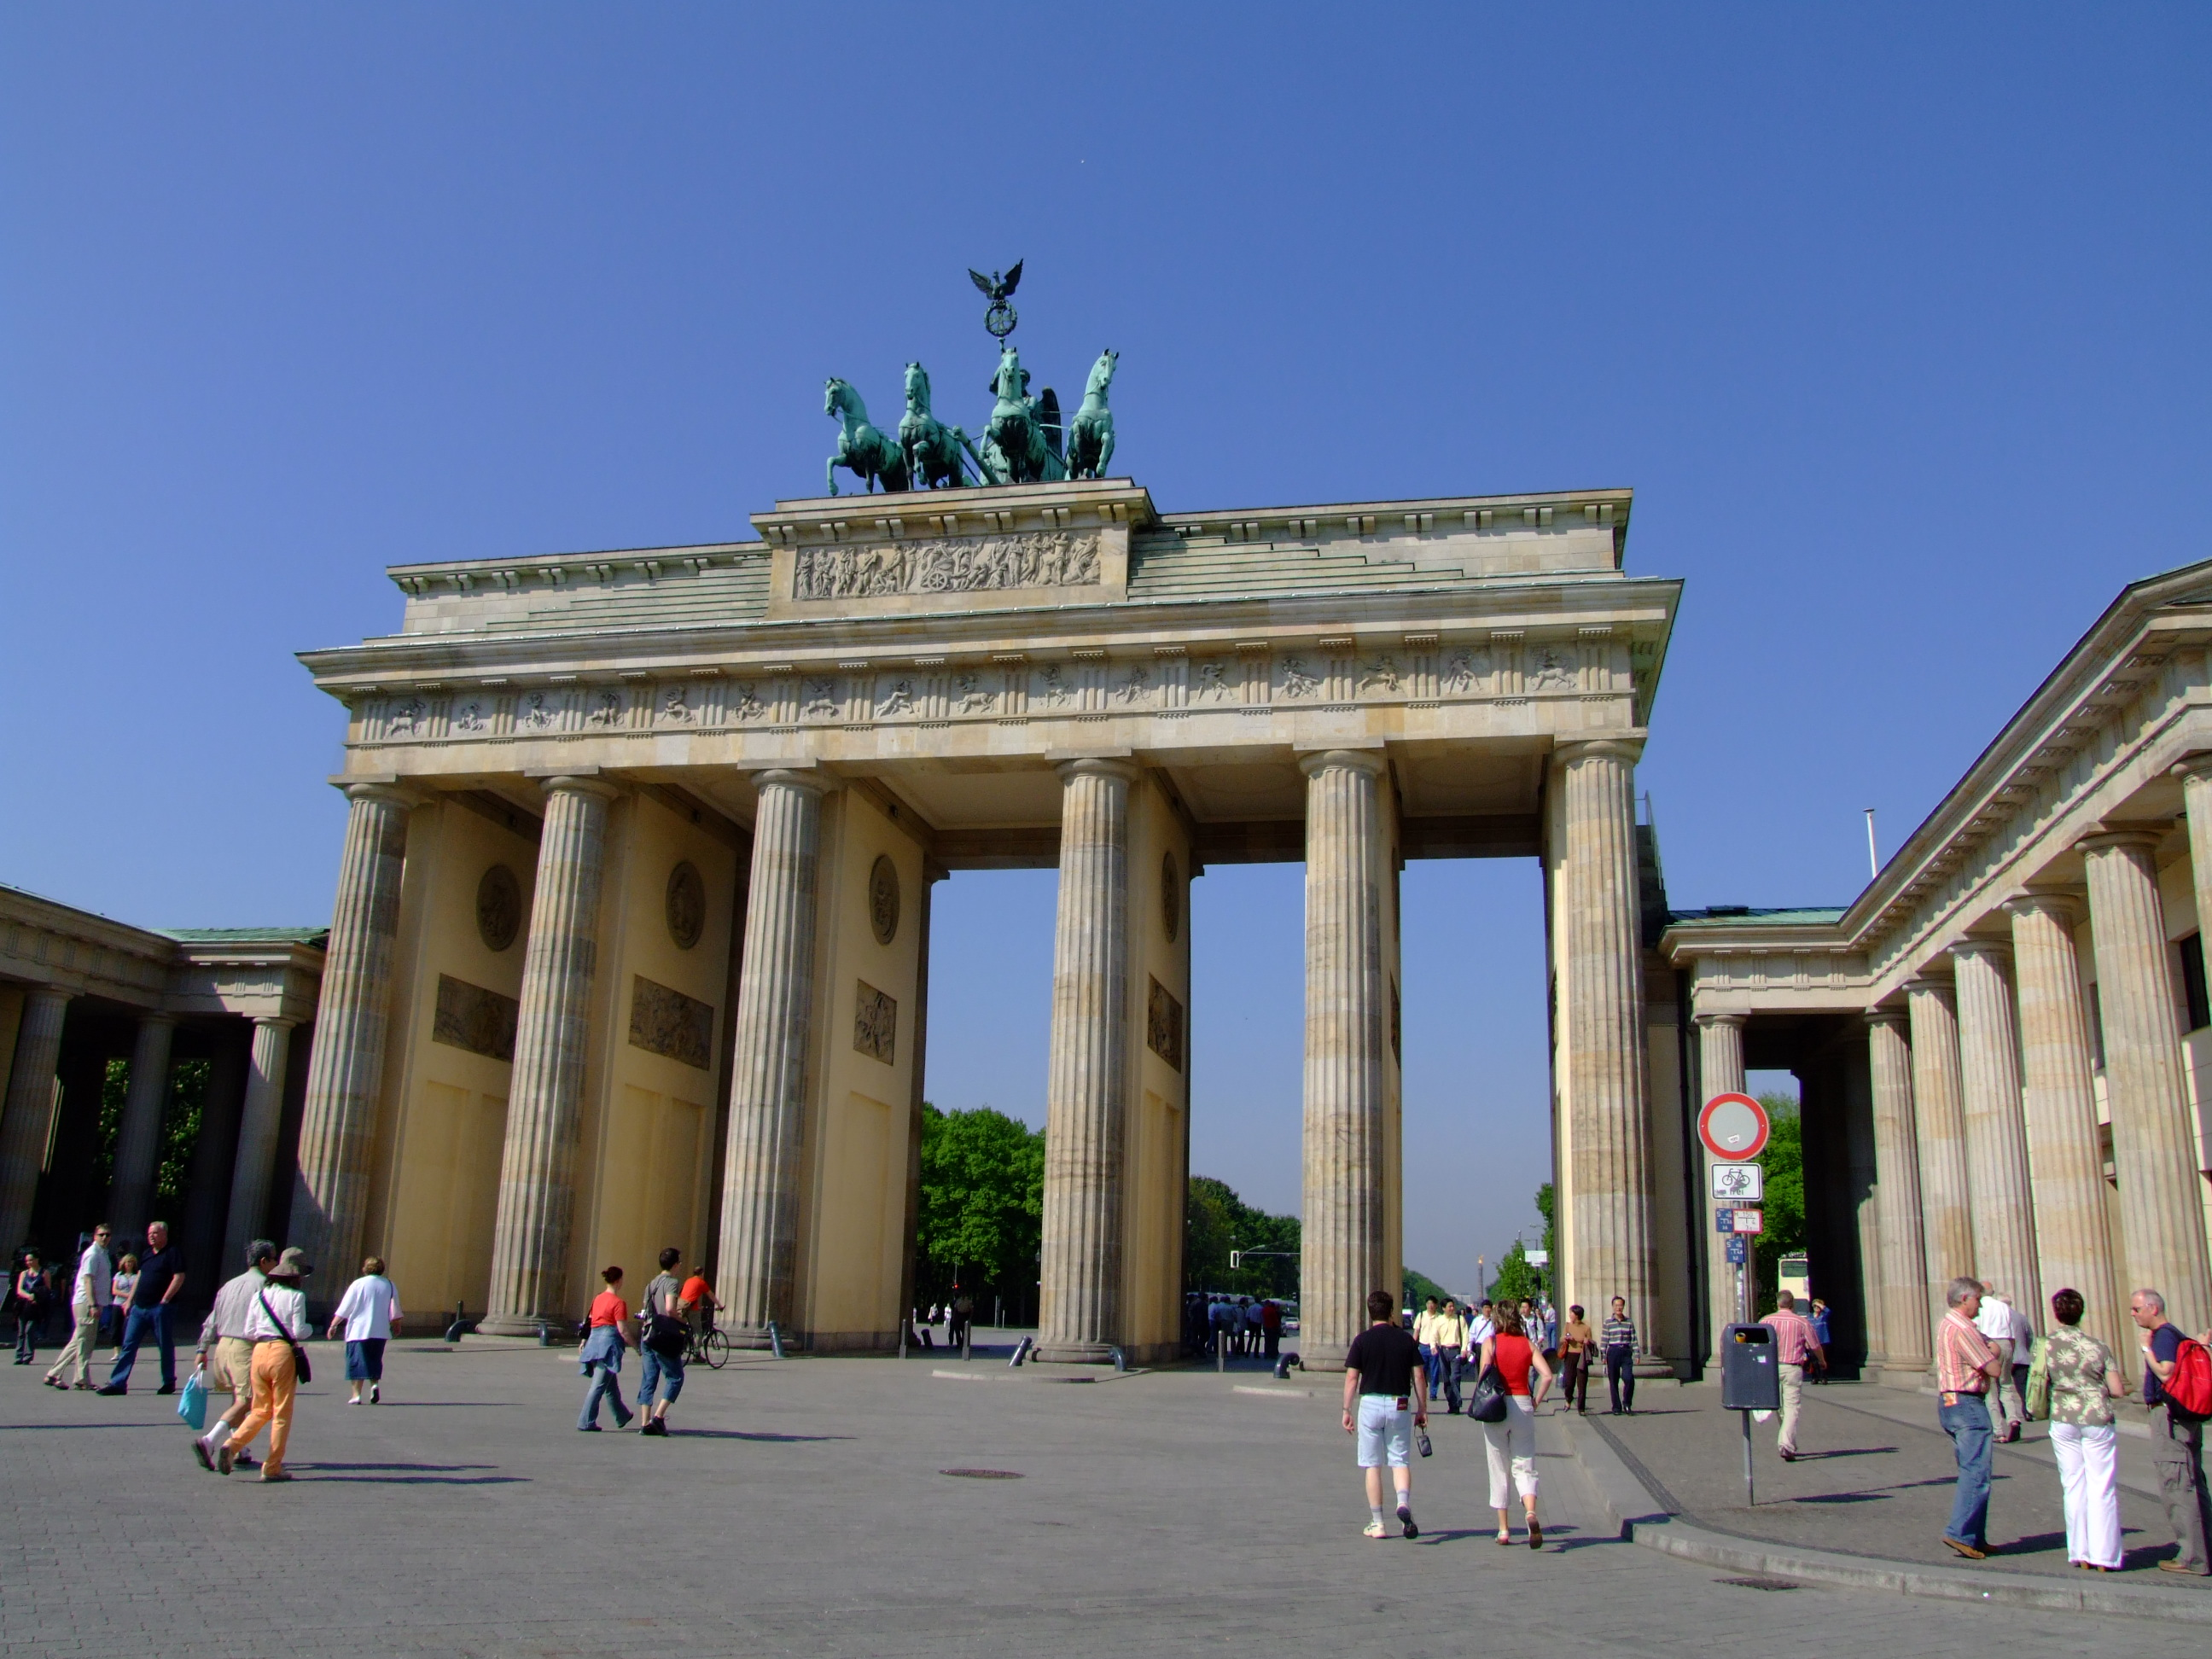
\includegraphics[width=190mm]{haupt}}
%\SetHorizontalCoffin \ethlogo {
\includegraphics[width=50mm]{logo}}
\SetHorizontalCoffin \textbox {\color{ethblue}\rule{190mm}{100mm}}
\SetVerticalCoffin \textboxtext {160mm} {\fontsize{40}{48}\mybold\noindent\textcolor{white}{\mytitle}}
%\SetVerticalCoffin \textboxsubtext {160mm} {\fontsize{21}{25}\dinproregular\noindent\textcolor{white}{MSc Thesis \\ Month Year}}
\SetVerticalCoffin \authortext {160mm} {\flushright\fontsize{21}{25}\myregular\noindent\textcolor{white}{\mytext}}
\SetHorizontalCoffin \departmentlogo {
\includegraphics[width=30mm]{logo}}

% Positioning Hax
\JoinCoffins \result \topbox
\JoinCoffins \result[\topbox-hc, \topbox-b] \imagebox [hc, t](0mm,10mm)
\JoinCoffins \result[\imagebox-l, \imagebox-t] \ethlogo [l, b](0mm,5mm)
\JoinCoffins \result[\imagebox-l, \imagebox-b] \textbox [l, t](0mm,0mm)
\JoinCoffins \result[\textbox-hc, \textbox-t] \textboxtext [hc, t](-5mm, -5mm)
\JoinCoffins \result[\textboxtext-l, \textboxtext-b] \textboxsubtext [l, t](0mm, -5mm)
\JoinCoffins \result[\textbox-r, \textbox-b] \authortext [r, b](-5mm, 5mm)
\JoinCoffins \result[\textbox-l, \textbox-b] \departmentlogo [l, t](-5mm, -5mm)


% Generate the page
\thispagestyle{empty}
\newgeometry{left=0mm,bottom=0mm, top=0mm, right=0mm}
\noindent\TypesetCoffin \result
\restoregeometry
	\cleardoubleemptypage
		\begin{titlepage}
			\vspace*{6cm}
			\noindent
			\center
			\titlefont Lexikon der kuturellen \\  Unterschiede zwischen \\ Deutschland und China\par
			\null
			\vspace*{12.5cm}
			\noindent
			\hfill
			
			\begin{minipage}{\linewidth}
				\center{\printauthor}
			\end{minipage}
		\end{titlepage}
	\cleardoubleemptypage
	\renewcommand{\cftdot}{$\cdot$}
	\renewcommand\thefigure{\thesection-\arabic{figure}}
	\renewcommand\thetable{\thesection-\arabic{table}}
	\newcommand{\mypar}{\par\noindent}
	\setlength\parskip{0.7em}
	\makeatletter
	\@addtoreset{table}{section}
	\makeatother
	\makeatletter
	\@addtoreset{figure}{section}
	\makeatother
	
	\pagestyle{empty}
	\begin{minipage}{\linewidth}
	\Huge\rmfamily\center {Zu diesem Buch} \par
\end{minipage}

 \vspace*{3cm}
 %\normalfont\normalsize
 %\justify
 \mypar
Sowohl China als auch Deutschland sind L\"ander mit einem bedeutenden Einfluss auf der Welt. Mit der Verbesserung der Kommunikationstechnologie, der Weiterentwicklung der Transporttechnologie und der starken Globalisierung der Wirtschaft ist die Zusammenarbeit zwischen den beiden Ländern immer häufiger geworden. Aufgrund des unterschiedlichen kulturellen Hintergrunds können sich die Menschen der beiden Länder jedoch nicht während des Geschlechtsverkehrs verstehen und die Kommunikation kann nicht reibungslos durchgeführt werden. Angesichts der immer häufiger werdenden Austauschaktivitäten zwischen CDAI und der Deutschen Fachhochschule hoffen wir, einige der Informationen, die wir für die Studenten beider L\"ander so gut wie möglich kennen und ordnen, zu ordnen und zu klassifizieren. Einige Tipps. Dieses Buch soll nicht allumfassend sein, aber es ist genau, detailliert und interessant. Diese Broschüre soll nicht allumfassend sein, aber es ist genau, detailliert und interessant.
\mypar
Das Chinesisch-Deutschen Institut für Angewandte Ingenieurwissenschaften (CDAI) wurde Anfang Mai im Rahmen eines Treffens von Vertretern der Fachhochschulen Lübeck und Westküste und der Zhejiang University for Science and Technology (ZUST) gestartet. Das CDAI ist in die langjährige erfolgreiche Partnerschaft des Landes Schleswig-Holsteins mit der Provinz Zhejiang eingebettet. Im Fokus des Instituts stehen anwendungsorientierten Bachelor-Ingenieurstudiengänge der schleswig-holsteinischen Fachhochschulen: – Management und Technik der FH Westküste in Heide sowie – Bauingenieurwesen der FH Lübeck. Ca. ein Drittel der fachlichen Lehrveranstaltungen in Hangzhou werden von der jeweiligen Mutterhochschule unterstützt. Die Unterrichtssprache ist zunächst Chinesisch, ab dem dritten Semester kommt Deutsch hinzu und ab dem dritten Studienjahr wird komplett auf Deutsch unterrichtet. Den erfolgreichen Teilnehmern der Studiengänge winkt ein deutscher und ein chinesischer Bachelorabschluss. Für die besten Studierenden besteht die Möglichkeit, im zweiten Studienabschnitt für drei Semester an die jeweilige deutsche Fachhochschule zu wechseln, um das Studium dort zu beenden. Im Gegenzug sollen deutsche Studierende aus dem entsprechenden Studiengang der Partnerhochschule einen Teil ihres Studiums in Hangzhou absolvieren.

\mypar
Im letzten Semester förderten wir unter Leitung von Projektsponsorin Frau Schneider den kulturelle Verstand zwischen chinesischen und deutschen Studenten in CDAI und deutsche partnerschaftliche Fachhochschule, die durch kulturelle Unterschiede verursacht wurden. Gleichzeitig wurden eine Reihe von Seminaren, Interviews, Fragebögen und Untersuchungen vor Ort zu den kulturellen Unterschieden durchgeführt, um sich an den internationalen Unterrichtsstil und das diversifizierte humanistische Umfeld anzupassen und zu integrieren.  Endlich konzentriert die Perspektive sich auf sieben kulturelle Themen: Kleidung, Ernährung, Sport, Arbeit, Transport, Kultur und Gesundheit und Schreiben wir eine Wikibasiertes Webseite.Aus Sicht der Studenten zeigen wir einmalig unser Verständnis und Denken über fremde Kulturen. Während des Projekts haben wir das Wissen des Projektmanagements voll genutzt und den Projektprozess durch Projektmanagement-Tools wie Projektauftrag, Zeitplan, PSP gesteuert, durch Absprache mit relevanten Materialien, Austausch mit deutschen Lehrern und Schülern und nach der tatsächlichen Lebenserfahrung bestimmt. Die spezifischen Inhalte jedes Themas und zeigen regelmä\ss ig die Arbeitsergebnisse für Klassenkameraden und Lehrer. Am Ende des Projekts sind unsere Ergebnisse erfreulich: Unsere chinesisch-deutsche Enzyklopädie für kulturelle Unterschiede befindet sich auf der offiziellen Website des Kollegs und zeigt den chinesischen und deutschen Lehrern und Schülern einen Einblick in den chinesisch-deutschen Kulturgarten. Wir hoffen, dass durch die gemeinsamen Anstrengungen dieses Semesters die kulturelle Brücke zwischen China und Deutschland stärker und schöner wird.Verglichen mit dem letzten Semester beginnt dieses Semester mit den Unterschieden im täglichen Verhalten der Chinesen und Deutschen und analysiert die kulturellen Konnotationen der einzelnen Unterschiede. Wir hoffen, dass chinesische und deutsche Studenten durch diese Broschüre ihr Verständnis verbessern werden.

\mypar
In China gibt es eine kleine Geschichte. wenn es um die Han-Dynastie \footnote{Die Han-Dynastie regierte das Kaiserreich China von 206 v. Chr. bis 220 n. Chr. Man unterscheidet zwischen der Periode der Frühen Han (207 v. Chr.–6/9 n. Chr.) und der Späten Han (23/25–220), unterbrochen durch die Herrschaft des Wang Mang. } geht, gibt es ein kleines Land namens Yelang im Südwesten. Obwohl es ein unabhängiges Land ist, ist das Land klein, es gibt nur wenige Menschen und das Eigentum ist noch weniger. Aber in der  Nachbarregion ist Yelang das grö\ss te Land. der König von Yelang glaubt , der das Land nie verlassen hat, dass das Land, das er regierte, das grö\ss te Land der Welt ist. Als eines Tages der König des Königreichs Yelang und seine Männer das Land besuchten, zeigte er nach vorne und fragte: ''Welches Land ist hier das grö\ss te?'' die Untergebenen sagten : ''Natürlich ist Yelang grö\ss te L\"ander ''.   Bei einer Gelegenheit sandte die Han-Dynastie Boten nach Yelang . Der König fragte den Boten: „Ist die Han-Dynastie grö\ss er als mein Land?“ Der Bote war schockiert. er kannte nicht glaub, was König des kleine Land sagt besonders dass mit der Han-Dynastie vergleicht, weil das Land, das er regierte, nur ungefähr dasselbe war wie ein Landkreis in der Han-Dynastie. Im Kontext der Globalisierung sollte die chinesische Jugend heutzutage die Welt in kürzester Zeit betrachten. Deutschland ist eines der Wichtigsten Länder der Welt. Die deutsche Kultur kann nicht ignoriert werden. Angesichts des immer banaleren Austausches zwischen China und Deutschland ist es auch sinnvoll f\"ur die deutsche Jugend über die chinesische Kultur zu kennen. Kurz gesagt, diese Broschüre möchte als Ausgangspunkt dienen, damit Studierende von beiden  L\"ander die Kultur des jeweils anderen verstehen können.Als chinesischer Student haben wir kein tieferes Verständnis für die deutsche Kultur, wir hoffen Sie wertvolle Anregungen zu geben, wenn Sie dieses Buch gelesen haben .
\vspace{\baselineskip}
\begin{flushright}\noindent
HangZhou, Mai.  2019\hfill {\texttt Alle Mitgliede des Projekt4}\\
\end{flushright}

	\pagestyle{scrheadings} 
	\tableofcontents
	\cleardoubleemptypage
	\input{Chapter_DE}
\end{document}